\documentclass[11pt,a4paper]{article}
\usepackage[margin=2cm]{geometry}
\usepackage{amsmath,amssymb,amsthm}
\usepackage{booktabs}
\usepackage{enumitem}
\usepackage{hyperref}
\usepackage{tikz}
\usepackage{listings}
\usetikzlibrary{arrows.meta,positioning,shapes.geometric,calc,fit,backgrounds,decorations.pathreplacing}

\newcommand{\RR}{\mathbb{R}}
\newcommand{\1}{\mathbf{1}}
\DeclareMathOperator{\sign}{sign}
\DeclareMathOperator{\sigmoid}{sigmoid}
\DeclareMathOperator{\logsumexp}{logsumexp}

\lstset{
  basicstyle=\ttfamily\small,
  breaklines=true,
  frame=single,
  backgroundcolor=\color{gray!5},
}

\title{SATA Synthetic Experiment Pipeline\\[4pt]
       \large Implementation Specification for Bug-Hunting}
\author{SATA Project --- Honours Thesis}
\date{September 2026}

\begin{document}
\maketitle
\tableofcontents
\newpage

%======================================================================
\part{Data Generation}
%======================================================================

%======================================================================
\section{Overview}
%======================================================================

The generator produces synthetic binary-classification tasks with \emph{known
ground truth}, so that we can precisely control which distribution shift is
applied and measure whether an LLM's in-context learning (ICL) is affected
by different demo-selection strategies.

Two independent axes define every dataset:
\begin{enumerate}
  \item \textbf{Rule family} --- how labels are generated from features
        (linear, threshold, tree, sparse\_interaction).
  \item \textbf{Environment / shift type} --- how the OOD test set differs
        from the ID data (covariate, mechanism, spurious\_reversal,
        extrapolation, missing\_feature).
\end{enumerate}

The same set of tasks is reused across all three primary datasets; only the
OOD environment changes.

%----------------------------------------------------------------------
\subsection{End-to-End Pipeline}
%----------------------------------------------------------------------

\begin{center}
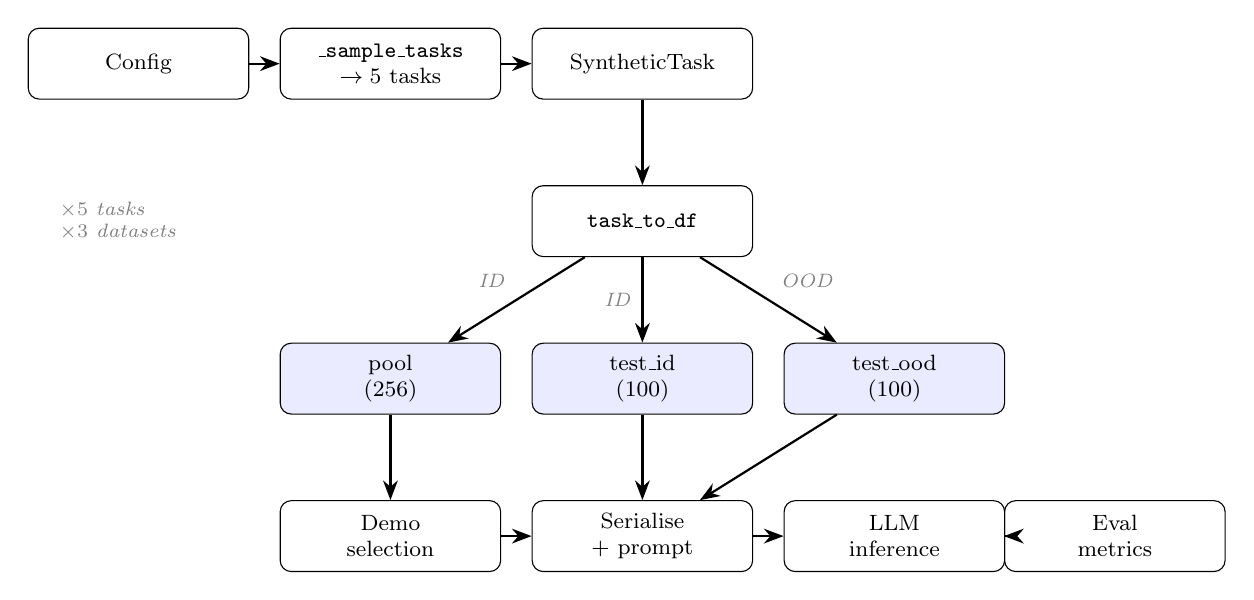
\begin{tikzpicture}[
    box/.style={draw, rounded corners, minimum width=2.8cm,
                minimum height=0.9cm, align=center, font=\footnotesize},
    data/.style={box, fill=blue!8},
    arrow/.style={-{Stealth[length=2.5mm]}, thick},
    lbl/.style={font=\scriptsize\itshape, text=gray},
    every node/.style={inner sep=4pt},
  ]
  % Row 1
  \node[box] (config) at (0,0) {Config};
  \node[box] (sample) at (3.2,0) {\texttt{\_sample\_tasks}\\$\to 5$ tasks};
  \node[box] (task) at (6.4,0) {SyntheticTask};

  \draw[arrow] (config) -- (sample);
  \draw[arrow] (sample) -- (task);

  % Row 2
  \node[box] (t2df) at (6.4,-2) {\texttt{task\_to\_df}};
  \draw[arrow] (task) -- (t2df);

  % Outputs
  \node[data] (pool) at (3.2,-4) {pool\\(256)};
  \node[data] (tid) at (6.4,-4) {test\_id\\(100)};
  \node[data] (tood) at (9.6,-4) {test\_ood\\(100)};

  \draw[arrow] (t2df) -- (pool) node[midway, above left, lbl] {ID};
  \draw[arrow] (t2df) -- (tid) node[midway, left, lbl] {ID};
  \draw[arrow] (t2df) -- (tood) node[midway, above right, lbl] {OOD};

  \node[lbl, text width=2cm] at (0,-2) {$\times 5$ tasks\\$\times 3$ datasets};

  % Row 3 -- downstream
  \node[box] (select) at (3.2,-6) {Demo\\selection};
  \node[box] (serial) at (6.4,-6) {Serialise\\+ prompt};
  \node[box] (infer) at (9.6,-6) {LLM\\inference};
  \node[box] (eval) at (12.4,-6) {Eval\\metrics};

  \draw[arrow] (pool) -- (select);
  \draw[arrow] (select) -- (serial);
  \draw[arrow] (tid) -- (serial);
  \draw[arrow] (tood) -- (serial);
  \draw[arrow] (serial) -- (infer);
  \draw[arrow] (infer) -- (eval);
\end{tikzpicture}
\end{center}

%======================================================================
\section{Configuration Parameters (NB01)}
%======================================================================

\begin{center}
\begin{tabular}{lll}
\toprule
\textbf{Parameter} & \textbf{Value} & \textbf{Meaning} \\
\midrule
\texttt{n\_features}             & 10              & Total columns: $f_0,\ldots,f_9$ \\
\texttt{n\_causal\_range}        & $[3, 5]$        & $n_{\text{causal}} \sim \text{U}\{3,4,5\}$ \\
\texttt{rule\_families}          & linear, threshold, tree & Sampled uniformly \\
\texttt{spurious\_strength\_range}& $[0.80, 0.90]$ & $s \sim \text{U}(0.80, 0.90)$ \\
\texttt{label\_noise}            & 0.02            & $P(\text{flip}) = 0.02$ \\
\texttt{coefficient\_scale}      & 1.5             & $c_j \sim \mathcal{N}(0, 1.5^2)$ \\
\texttt{N\_TASKS}                & 5               & Tasks per experiment \\
\texttt{N\_POOL}                 & 256             & Demo candidate pool per task \\
\texttt{N\_TEST\_ID}             & 100             & ID test rows per task \\
\texttt{N\_TEST\_OOD}            & 100             & OOD test rows per task \\
\bottomrule
\end{tabular}
\end{center}

%======================================================================
\section{Feature Roles}
%======================================================================

Every row has 10 features:

\begin{center}
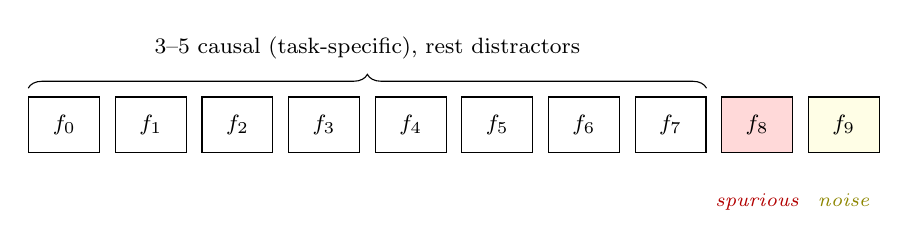
\begin{tikzpicture}[
    feat/.style={draw, minimum width=0.9cm, minimum height=0.7cm,
                 align=center, font=\footnotesize},
    spurious/.style={feat, fill=red!15},
    noise/.style={feat, fill=yellow!10},
  ]
  \foreach \i in {0,...,7} {
    \node[feat] (f\i) at (\i*1.1, 0) {$f_{\i}$};
  }
  \node[spurious] (f8) at (8*1.1, 0) {$f_8$};
  \node[noise] (f9) at (9*1.1, 0) {$f_9$};

  \draw[decorate, decoration={brace, amplitude=5pt, raise=3pt}]
    (f0.north west) -- (f7.north east)
    node[midway, above=10pt, font=\footnotesize]
    {3--5 causal (task-specific), rest distractors};

  \node[below=0.4cm of f8, font=\scriptsize\itshape, text=red!70!black] {spurious};
  \node[below=0.4cm of f9, font=\scriptsize\itshape, text=olive] {noise};
\end{tikzpicture}
\end{center}

\begin{itemize}[nosep]
  \item $f_0$--$f_7$: drawn $\sim \mathcal{N}(0,1)$. A task-specific subset
        (3--5) is \emph{causal}; the rest are distractors.
  \item $f_8$: \textbf{spurious}, generated \emph{from} the label
        (Section~\ref{sec:spurious}). Not used by any rule.
  \item $f_9$: \textbf{pure noise}, $\sim \mathcal{N}(0,1)$, independent of
        everything.
\end{itemize}

%======================================================================
\section{Task Sampling: \texttt{\_sample\_tasks()}}
\label{sec:sample-tasks}
%======================================================================

For each of the $N=5$ tasks, sampled independently:

\begin{enumerate}[nosep]
  \item \textbf{Rule family:}
        $\text{family} \sim \text{Uniform}\{\text{linear},\;
        \text{threshold},\;\text{tree}\}$

  \item \textbf{Number of causal features:}
        $n_{\text{causal}} \sim \text{U}\{3,4,5\}$

  \item \textbf{Causal feature indices:}
        $n_{\text{causal}}$ distinct indices from $\{0,\ldots,7\}$, sorted.

  \item \textbf{Coefficients} (used only by linear, sampled for all
        families for RNG consistency):
        $c_j \sim \mathcal{N}(0,\; 1.5^2)$

  \item \textbf{Spurious strength:}
        $s \sim \text{U}(0.80,\; 0.90)$

  \item \textbf{Family-specific:}
        \begin{itemize}[nosep]
          \item \texttt{threshold}: $k{=}\min(3, n_{\text{causal}})$ thresholds,
                $t_j \sim \text{U}(-0.3,\; 0.3)$.
          \item \texttt{tree}: $k{=}\min(3, n_{\text{causal}})$ leaf labels via
                \texttt{\_sample\_tree\_leaf\_labels(k)}
                (Section~\ref{sec:tree-labels}).
          \item \texttt{sparse\_interaction}: threshold from a
                10k-sample probe targeting base rate $\sim \text{U}(0.35, 0.65)$.
        \end{itemize}
\end{enumerate}

%======================================================================
\section{Rule Families: \texttt{\_apply\_rule()}}
\label{sec:rules}
%======================================================================

Given $X \in \RR^{n \times 10}$ and optional $u \in [0,1]^n$, compute
$y_{\text{clean}} \in \{0,1\}^n$:

%----------------------------------------------------------------------
\subsection{Linear}
%----------------------------------------------------------------------

\[
  \text{logit}_i = \mathbf{c}^\top \mathbf{X}_{i,\,\text{causal}},
  \qquad
  p_i = \sigmoid(\text{logit}_i) = \frac{1}{1 + e^{-\text{logit}_i}}
\]
\[
  y_{\text{clean},i} =
  \begin{cases}
    \1[u_i < p_i] & \text{stochastic (data generation)} \\
    \1[p_i > 0.5] & \text{MAP (probes)}
  \end{cases}
\]

\textit{Why stochastic?} A deterministic rule is scale-invariant, making the
causal signal perfectly reliable at any coefficient scale. Bernoulli sampling
introduces concept noise so the spurious feature can compete.

%----------------------------------------------------------------------
\subsection{Threshold (Majority Vote)}
%----------------------------------------------------------------------

$k = \min(3, n_{\text{causal}})$, thresholds $t_1, t_2, t_3$:
\[
  b_{i,j} = \1\bigl[X_{i,\,\text{causal}_j} > t_j\bigr],
  \qquad
  y_{\text{clean},i} = \1\!\left[\sum_{j=1}^{k} b_{i,j} \geq 2\right]
\]

%----------------------------------------------------------------------
\subsection{Tree (Depth-3)}
\label{sec:tree}
%----------------------------------------------------------------------

$k = \min(3, n_{\text{causal}})$, giving $2^k$ leaves:
\[
  \text{leaf\_id}_i = \sum_{j=0}^{k-1}
  \1\bigl[X_{i,\,\text{causal}_j} > 0\bigr] \cdot 2^j,
  \qquad
  y_{\text{clean},i} = \text{leaf\_labels}[\text{leaf\_id}_i]
\]

\subsubsection{Tree Leaf Label Sampling}
\label{sec:tree-labels}

Two constraints:
\begin{enumerate}[nosep]
  \item \textbf{Complement antisymmetry:}
        $\text{leaf\_labels}[L] = 1 - \text{leaf\_labels}[2^k{-}1{-}L]$.
        Guarantees mechanism's sign flip always inverts the label.
  \item \textbf{Non-degeneracy} ($k \geq 3$): Reject dictator (single-bit)
        and parity (XOR-of-all-bits) functions.
\end{enumerate}

%----------------------------------------------------------------------
\subsection{Sparse Interaction}
%----------------------------------------------------------------------

\[
  y_{\text{clean}} = \1\bigl[X_{:,\,i} \cdot X_{:,\,j} > \theta\bigr]
\]
Only the first two causal features participate; the rest are decoys.

%======================================================================
\section{Environment Generation: \texttt{generate\_environment()}}
\label{sec:environments}
%======================================================================

Every call follows the same skeleton:

\begin{center}
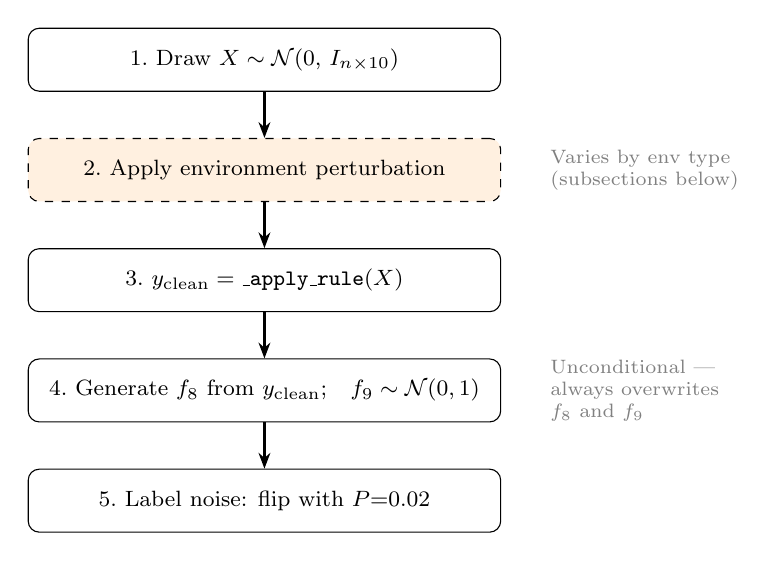
\begin{tikzpicture}[
    stp/.style={draw, rounded corners, minimum width=6cm,
                 minimum height=0.8cm, align=center, font=\footnotesize},
    perturb/.style={stp, fill=orange!12, dashed},
    arrow/.style={-{Stealth[length=2mm]}, thick},
    note/.style={font=\scriptsize, text=gray, align=left},
  ]
  \node[stp]     (s1) at (0, 0)    {1.\ Draw $X \sim \mathcal{N}(0,\,I_{n\times 10})$};
  \node[perturb] (s2) at (0,-1.4)  {2.\ Apply environment perturbation};
  \node[stp]     (s3) at (0,-2.8)  {3.\ $y_{\text{clean}} = \texttt{\_apply\_rule}(X)$};
  \node[stp]     (s4) at (0,-4.2)  {4.\ Generate $f_8$ from $y_{\text{clean}}$;\quad $f_9 \sim \mathcal{N}(0,1)$};
  \node[stp]     (s5) at (0,-5.6)  {5.\ Label noise: flip with $P{=}0.02$};

  \draw[arrow] (s1) -- (s2);
  \draw[arrow] (s2) -- (s3);
  \draw[arrow] (s3) -- (s4);
  \draw[arrow] (s4) -- (s5);

  \node[note, right=0.5cm of s2] {Varies by env type\\(subsections below)};
  \node[note, right=0.5cm of s4] {Unconditional ---\\always overwrites\\$f_8$ and $f_9$};
\end{tikzpicture}
\end{center}

%----------------------------------------------------------------------
\subsection{\texorpdfstring{\texttt{id}}{id} --- In-Distribution}
%----------------------------------------------------------------------

No perturbation. $X$, $\mathbf{c}$, $s$ unchanged.

%----------------------------------------------------------------------
\subsection{\texorpdfstring{\texttt{covariate}}{covariate} --- $P(X)$ Shift}
\label{sec:covariate}
%----------------------------------------------------------------------

Shift $P(X)$ while preserving $P(Y)$:

\begin{enumerate}[nosep]
  \item Estimate unshifted base rate
        $r_{\text{id}} = \hat{P}(y{=}1)$ via 2048-row probe.

  \item \textbf{Rejection loop} (up to 50 iterations):
        \begin{enumerate}[nosep,label=(\alph*)]
          \item Sample 3 features from $\{0,\ldots,7\}$ without replacement.
          \item Sample deltas:
                $\delta_j \sim \text{U}(1,2) \times \text{Rademacher}$
                (so $\delta_j \in [-2,-1]\cup[1,2]$).
          \item Probe shifted base rate $r_{\text{shifted}}$.
          \item Accept if $|r_{\text{shifted}} - r_{\text{id}}| \leq 0.03$.
        \end{enumerate}

  \item Apply: $X_{:,\,\text{feats}} \mathrel{+}= \delta$.
\end{enumerate}

Features 8, 9 excluded (overwritten later).

%----------------------------------------------------------------------
\subsection{\texorpdfstring{\texttt{mechanism}}{mechanism} --- $P(Y|X)$ Shift}
\label{sec:mechanism}
%----------------------------------------------------------------------

\begin{enumerate}[nosep]
  \item Rescale coefficients:
        $c'_j = c_j \cdot u_j,\; u_j \sim \text{U}(0.5, 1.5)$
  \item Sign-flip causal features (on a copy):
        $\tilde{X}_{:,\text{causal}} = -X_{:,\text{causal}}$
\end{enumerate}

The rule operates on $\tilde{X}$ with $c'$; the returned $X$ is unchanged.
The LLM sees original features but shifted labels.

\textbf{Note on $f_8$:} Generated from $y_{\text{clean}}$ \emph{after} the
mechanism flip, so $f_8$ tracks the \emph{new} ground truth at strength $s$.

%----------------------------------------------------------------------
\subsection{\texorpdfstring{\texttt{spurious\_reversal}}{spurious-reversal} --- Spurious Flip}
\label{sec:spurious-reversal}
%----------------------------------------------------------------------

One line: $s' = 1 - s$. Everything else unchanged. $P(\text{agreement})$
drops from ${\sim}0.85$ to ${\sim}0.15$.

%----------------------------------------------------------------------
\subsection{\texorpdfstring{\texttt{extrapolation}}{extrapolation} --- Out-of-Support}
%----------------------------------------------------------------------

Replace 2--3 causal features per row:
$X_{i,f} = s_i \cdot m_i$, \;
$m_i \sim \text{U}(2,4)$, \;
$s_i \sim \text{Rademacher}$.

%----------------------------------------------------------------------
\subsection{\texorpdfstring{\texttt{missing\_feature}}{missing-feature} --- Broken Measurement}
%----------------------------------------------------------------------

$X_{:,\,\text{causal}[0]} \leftarrow \mathcal{N}(0,1)$ (fresh, independent of label).

%======================================================================
\section{Spurious Feature Construction ($f_8$)}
\label{sec:spurious}
%======================================================================

\[
  d = \Phi^{-1}(s), \qquad
  X_{i,8} = (2\,y_{\text{clean},i} - 1) \cdot d + \varepsilon_i,
  \quad \varepsilon_i \sim \mathcal{N}(0, 1)
\]

\textbf{Distribution by label:}
\begin{align*}
  y = 1 &\implies X_8 \sim \mathcal{N}(+d,\; 1) \\
  y = 0 &\implies X_8 \sim \mathcal{N}(-d,\; 1)
\end{align*}

\textbf{Sign-agreement:}
For $y=1$: $P(X_8 > 0) = P(Z > -d) = \Phi(d) = s$.
For $y=0$: $P(X_8 < 0) = P(Z < d) = \Phi(d) = s$.

Under spurious reversal: $d' = \Phi^{-1}(1-s) = -d$, so
$P(\text{agreement}) = 1 - s$.

%======================================================================
\section{Label Noise}
%======================================================================

\[
  y_i = \begin{cases}
    1 - y_{\text{clean},i} & \text{w.p.\ } \eta = 0.02 \\
    y_{\text{clean},i}     & \text{w.p.\ } 1 - \eta
  \end{cases}
\]

$f_8$ is generated from $y_{\text{clean}}$ (pre-noise), not $y$ (post-noise).

%======================================================================
\section{Dataset Construction: \texttt{task\_to\_dataframes()}}
\label{sec:datasets}
%======================================================================

For one task and one OOD environment:

\begin{center}
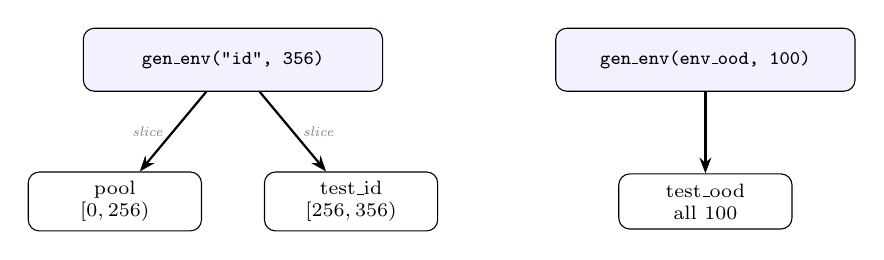
\begin{tikzpicture}[
    call/.style={draw, rounded corners, minimum width=3.8cm,
                 minimum height=0.8cm, align=center, font=\scriptsize,
                 fill=blue!5},
    split/.style={draw, rounded corners, minimum width=2.2cm,
                  minimum height=0.7cm, align=center, font=\scriptsize},
    arrow/.style={-{Stealth[length=2mm]}, thick},
    lbl/.style={font=\tiny\itshape, text=gray},
  ]
  \node[call] (id) at (0,0) {\texttt{gen\_env("id", 356)}};
  \node[call] (ood) at (6,0) {\texttt{gen\_env(env\_ood, 100)}};

  \node[split] (pool) at (-1.5,-1.8) {pool\\$[0, 256)$};
  \node[split] (tid) at (1.5,-1.8) {test\_id\\$[256, 356)$};
  \node[split] (tood) at (6,-1.8) {test\_ood\\all 100};

  \draw[arrow] (id) -- (pool) node[midway, left, lbl] {slice};
  \draw[arrow] (id) -- (tid) node[midway, right, lbl] {slice};
  \draw[arrow] (ood) -- (tood);
\end{tikzpicture}
\end{center}

Repeated for 5 tasks $\times$ 3 datasets. Each dataset uses a different OOD:

\begin{center}
\begin{tabular}{lll}
\toprule
\textbf{Dataset} & \textbf{\texttt{env\_ood}} & \textbf{What shifts} \\
\midrule
\texttt{synth\_covariate} & \texttt{covariate}          & $P(X)$ \\
\texttt{synth\_concept}   & \texttt{mechanism}          & $P(Y|X)$ \\
\texttt{synth\_spurious}  & \texttt{spurious\_reversal} & $f_8$ correlation \\
\bottomrule
\end{tabular}
\end{center}

Sizes per dataset: pool = $5 \times 256 = 1280$, test\_id = 500, test\_ood = 500.

%======================================================================
\section{Causal Graph}
%======================================================================

\begin{center}
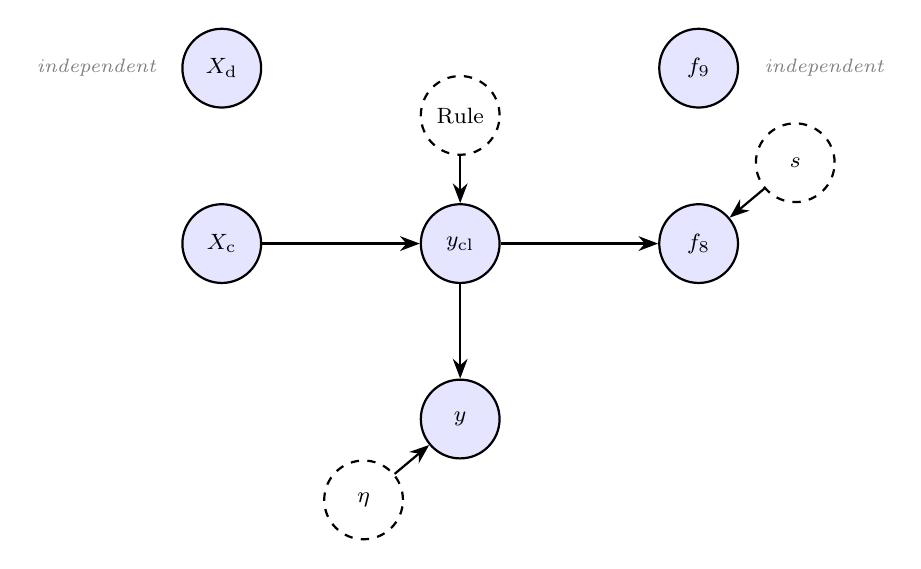
\begin{tikzpicture}[
    node distance=1.5cm,
    var/.style={draw, circle, minimum size=1cm, font=\footnotesize, thick},
    obs/.style={var, fill=blue!10},
    hidden/.style={var, dashed},
    arrow/.style={-{Stealth[length=2.5mm]}, thick},
    lbl/.style={font=\scriptsize\itshape, text=gray},
  ]
  \node[obs] (Xc) {$X_{\text{c}}$};
  \node[obs, right=2cm of Xc] (yclean) {$y_{\text{cl}}$};
  \node[obs, right=2cm of yclean] (f8) {$f_8$};
  \node[obs, below=1.2cm of yclean] (y) {$y$};
  \node[obs, above=1.2cm of Xc] (Xd) {$X_{\text{d}}$};
  \node[obs, above=1.2cm of f8] (f9) {$f_9$};

  \node[hidden, above=0.6cm of yclean] (rule) {Rule};
  \node[hidden, above right=0.3cm and 0.5cm of f8] (s) {$s$};
  \node[hidden, below left=0.3cm and 0.5cm of y] (eta) {$\eta$};

  \draw[arrow] (Xc) -- (yclean);
  \draw[arrow] (rule) -- (yclean);
  \draw[arrow] (yclean) -- (f8);
  \draw[arrow] (s) -- (f8);
  \draw[arrow] (yclean) -- (y);
  \draw[arrow] (eta) -- (y);

  \node[lbl, left=0.2cm of Xd] {independent};
  \node[lbl, right=0.2cm of f9] {independent};
\end{tikzpicture}
\end{center}

\[
  X_{\text{causal}} \xrightarrow{\text{rule}} y_{\text{clean}}
  \xrightarrow{(2y{-}1)d + \varepsilon} f_8
\]

$f_8$ is a \emph{descendant} of $y$, not a cause.

%======================================================================
\newpage
\part{Downstream Pipeline}
%======================================================================

%======================================================================
\section{Demo Selection (NB02)}
\label{sec:selection}
%======================================================================

All selection functions return \texttt{list[int]} --- indices into the pool
DataFrame. $K = 8$ demos per query.

%----------------------------------------------------------------------
\subsection{Zero-Shot}
%----------------------------------------------------------------------

No demos selected. The LLM receives only the system instruction and query.

%----------------------------------------------------------------------
\subsection{Random}
%----------------------------------------------------------------------

$K$ indices sampled uniformly without replacement from the pool:
\[
  \text{demos} \sim \text{Uniform}(\text{pool.index},\; K)
\]

%----------------------------------------------------------------------
\subsection{Similarity}
%----------------------------------------------------------------------

Each pool row and query are serialised to text, then encoded via
\texttt{all-MiniLM-L6-v2} sentence embeddings (normalised).
Cosine similarity is a dot product:
\[
  \text{sim}_j = \mathbf{e}_{\text{pool}_j}^\top \mathbf{e}_{\text{query}},
  \qquad
  \text{demos} = \text{argsort}(-\text{sim})[:K]
\]

Pool embeddings are cached (keyed by hash of pool texts, max 64 entries).
Batch variant computes $Q \times P$ similarity matrix in one call.

%----------------------------------------------------------------------
\subsection{Label Diversity (Protocol A)}
%----------------------------------------------------------------------

Stratified sampling: $\lfloor K/2 \rfloor$ demos per class.
Remainder (if $K$ is odd) filled randomly from leftover pool.

%----------------------------------------------------------------------
\subsection{Feature Range (Protocol B)}
%----------------------------------------------------------------------

For up to 3 features from \texttt{top\_features} (ranked by mutual information):
\begin{enumerate}[nosep]
  \item Bin each feature into $n_{\text{bins}} = 3$ quantiles via \texttt{pd.qcut}.
  \item Form Cartesian cell key per row: $(\text{bin}_{f_1}, \text{bin}_{f_2}, \text{bin}_{f_3})$.
  \item Shuffle cells, sample 1 demo per cell until $K$ reached.
  \item Remainder filled randomly.
\end{enumerate}

%----------------------------------------------------------------------
\subsection{Rule Diversity (Protocol C)}
%----------------------------------------------------------------------

Two arms:
\begin{itemize}[nosep]
  \item \textbf{Real arm:} Fit a \texttt{max\_depth=3} decision tree on
        the pool; use \texttt{tree.apply()} to get leaf IDs as regime proxies.
  \item \textbf{Synthetic arm:} Use ground-truth \texttt{regime} from metadata.
\end{itemize}

Group pool rows by leaf/regime, shuffle groups, take 1 per group.

%----------------------------------------------------------------------
\subsection{Counter-Spurious (Protocol D)}
%----------------------------------------------------------------------

Two arms:
\begin{itemize}[nosep]
  \item \textbf{Synthetic arm:} Use ground-truth \texttt{is\_counter\_spurious}
        boolean from metadata.
  \item \textbf{Real arm:} Find proxy features by
        $\text{score}_f = |\text{corr}(f, \text{label})| \cdot |\text{corr}(f, \text{shift})|$.
        Identify ``minority cells'' where proxy--label correlation is broken.
\end{itemize}

Over-sample counter-spurious rows: $\lfloor K/2 \rfloor + 1$ from
counter-spurious indices, remainder from the rest.

%----------------------------------------------------------------------
\subsection{Ordering (Applied to All Methods)}
%----------------------------------------------------------------------

After selection, demo order is shuffled via a seeded permutation:
\[
  \text{ordered\_ids} = \pi_{\text{seed}}(\text{demo\_ids})
\]

This is a controlled nuisance variable (Lu et al., 2022): ordering effects
are uniform across all conditions.

%======================================================================
\section{Serialisation}
\label{sec:serialisation}
%======================================================================

Each row is converted to text via \texttt{serialise\_row()}:

\begin{lstlisting}
f0: 0.80; f1: -0.45; f2: -0.30; f3: 1.52; f4: -0.91;
f5: 1.10; f6: 0.07; f7: -1.33; f8: 0.64; f9: 0.22 -> 1
\end{lstlisting}

\textbf{Format:} \texttt{FeatureName: value; ... -> Label}

\begin{itemize}[nosep]
  \item Feature order: alphabetical by column name
        (\texttt{sorted(features.keys())}).
  \item Numeric values: fixed-width \texttt{f"\{v:.2f\}"} (2 decimal places).
  \item Query rows: end with \texttt{" ->"} (no label).
  \item NaN values: rendered as \texttt{"unknown"}.
  \item When codebook is provided: column names replaced by
        \texttt{name\_extended}, categorical codes replaced by
        human-readable labels.
\end{itemize}

%======================================================================
\section{Prompt Construction}
\label{sec:prompts}
%======================================================================

\texttt{build\_chat\_messages()} returns a 2-element message list:

\begin{enumerate}[nosep]
  \item \textbf{System message:}
        ``You are a classifier. Given the input features, predict the class.
        Respond with exactly one word: \texttt{0} or \texttt{1},
        where \texttt{0} = Class~0 and \texttt{1} = Class~1.''

  \item \textbf{User message:}
        Newline-joined demo lines (each with label), followed by the
        query line (no label).
\end{enumerate}

\texttt{ChatFormatter.render(system, user)} applies the model's chat template
(e.g.\ ChatML for Qwen) with special tokens and generation prompt:

\begin{lstlisting}
<|im_start|>system
You are a classifier. ...
<|im_end|>
<|im_start|>user
f0: 0.80; f1: -0.45; ... -> 1
f0: 1.20; f1: 0.33; ... -> 0
...
f0: -0.10; f1: 0.72; ... ->
<|im_end|>
<|im_start|>assistant
\end{lstlisting}

%======================================================================
\section{LLM Inference}
\label{sec:inference}
%======================================================================

Using \texttt{MLXRunner} (Apple Silicon, Qwen2.5-7B-Instruct).

%----------------------------------------------------------------------
\subsection{Forward Pass}
%----------------------------------------------------------------------

For each prompt, \texttt{\_next\_token\_logprobs(prompt)} performs:

\begin{enumerate}[nosep]
  \item Tokenise the full prompt string.
  \item Single forward pass through the model.
  \item Extract logits at the \emph{final} token position.
  \item Compute full-vocabulary log-probabilities:
        \[
          \ell_v = \text{logits}_v - \logsumexp(\text{logits})
        \]
\end{enumerate}

No sampling occurs; the model produces a probability distribution over
all tokens and we extract the two we care about.

%----------------------------------------------------------------------
\subsection{Prediction Extraction}
%----------------------------------------------------------------------

\texttt{get\_confidence(logprobs\_dict, label\_tokens)} computes:

\begin{enumerate}[nosep]
  \item Look up log-probs for the two label tokens:
        \[
          \ell_0 = \ell[\text{token}(\texttt{"0"})], \qquad
          \ell_1 = \ell[\text{token}(\texttt{"1"})]
        \]
        If a label token is absent from logprobs, default $\ell = -100$.

  \item \textbf{Constrained two-way softmax} (renormalise over label tokens only):
        \[
          p_0 = \frac{e^{\ell_0}}{e^{\ell_0} + e^{\ell_1}}, \qquad
          p_1 = 1 - p_0
        \]

  \item Prediction: $\hat{y} = \arg\max(p_0, p_1)$. \\
        Confidence: $\max(p_0, p_1)$.
\end{enumerate}

\textbf{Output:} \texttt{PredictionResult(prediction, confidence, p0, p1,
logprob\_0, logprob\_1)}.

If neither label token appears in logprobs $\to$ \texttt{INVALID}.

%======================================================================
\section{Evaluation Metrics}
\label{sec:evaluation}
%======================================================================

All metrics filter out \texttt{INVALID} predictions first. Predictions are
canonicalised: strip whitespace, convert numeric-looking strings to integers
(\texttt{"1.0"} $\to$ \texttt{"1"}).

%----------------------------------------------------------------------
\subsection{Accuracy}
%----------------------------------------------------------------------

\[
  \text{acc} = \frac{1}{|\mathcal{V}|}
  \sum_{i \in \mathcal{V}} \1[\hat{y}_i = y_i]
\]

where $\mathcal{V}$ is the set of non-INVALID predictions.
Returns NaN if $|\mathcal{V}| = 0$.

%----------------------------------------------------------------------
\subsection{Macro F1}
%----------------------------------------------------------------------

\[
  \text{F1}_{\text{macro}} = \frac{1}{C} \sum_{c=1}^{C} \text{F1}_c
  = \frac{1}{C} \sum_{c=1}^{C}
  \frac{2 \cdot \text{precision}_c \cdot \text{recall}_c}
       {\text{precision}_c + \text{recall}_c}
\]

Via \texttt{sklearn.metrics.f1\_score(..., average="macro")} on
canonicalised valid predictions.

%----------------------------------------------------------------------
\subsection{Shift Gap}
%----------------------------------------------------------------------

\[
  \Delta = \text{acc}_{\text{ID}} - \text{acc}_{\text{OOD}}
\]

Positive $\Delta$ indicates OOD degradation.

%----------------------------------------------------------------------
\subsection{Invalid Rate}
%----------------------------------------------------------------------

\[
  \text{inv} = \frac{|\{i : \hat{y}_i = \texttt{INVALID}\}|}{n}
\]

%======================================================================
\section{Experiment Orchestration (NB02)}
\label{sec:orchestration}
%======================================================================

\textbf{Parameters:} $K = 8$ demos, $N_{\text{queries}} = 30$ per
environment, seed = 42.

\textbf{Conditions:} zero\_shot, random, similarity, label\_diversity,
feature\_range, rule\_diversity, counter\_spurious (7 total).

\textbf{Per-dataset pre-computation:}
\begin{enumerate}[nosep]
  \item Load parquet files (pool, test\_id, test\_ood).
  \item \texttt{select\_top\_features(pool, n=3)} for feature\_range.
  \item \texttt{fit\_leaf\_tree(pool)} for rule\_diversity.
  \item \texttt{find\_spurious\_proxy\_features(pool $\cup$ test\_ood)} for
        counter\_spurious.
  \item Pre-compute similarity embeddings (batch).
\end{enumerate}

\textbf{Per-query data flow:}

\begin{center}
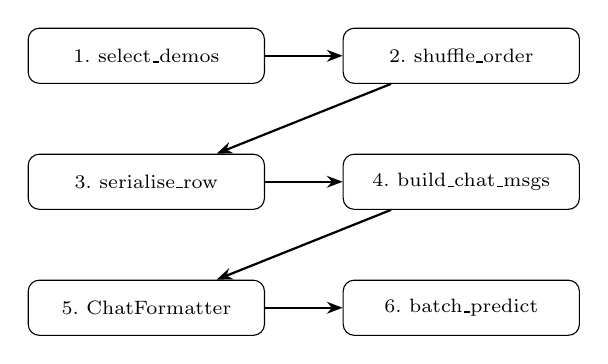
\begin{tikzpicture}[
    stp/.style={draw, rounded corners, minimum width=3cm,
                 minimum height=0.7cm, align=center, font=\scriptsize},
    arrow/.style={-{Stealth[length=2mm]}, thick},
  ]
  \node[stp] (s1) at (0,0) {1.\ select\_demos};
  \node[stp] (s2) at (4,0) {2.\ shuffle\_order};
  \node[stp] (s3) at (0,-1.6) {3.\ serialise\_row};
  \node[stp] (s4) at (4,-1.6) {4.\ build\_chat\_msgs};
  \node[stp] (s5) at (0,-3.2) {5.\ ChatFormatter};
  \node[stp] (s6) at (4,-3.2) {6.\ batch\_predict};

  \draw[arrow] (s1) -- (s2);
  \draw[arrow] (s2) -- (s3);
  \draw[arrow] (s3) -- (s4);
  \draw[arrow] (s4) -- (s5);
  \draw[arrow] (s5) -- (s6);
\end{tikzpicture}
\end{center}

All prompts for a condition are batched, then
\texttt{runner.batch\_predict(prompts, ("0", "1"))} runs them through MLX.
Results are scored per environment with accuracy, macro\_f1, invalid\_rate.

%======================================================================
\newpage
\part{Bug-Hunting Notes}
%======================================================================

\begin{enumerate}
  \item \textbf{$f_8$ is present in ALL environments (including ID).}
        The spurious correlation is part of the data-generating process.
        Only \texttt{synth\_spurious} tests reliance on $f_8$ by reversing it.

  \item \textbf{$f_8$ is a ``safety net'' in covariate and concept shifts.}
        In these datasets, $f_8$'s strength is unchanged between ID and OOD.
        In \texttt{synth\_concept}, $f_8$ tracks the \emph{new} ground truth
        (generated after the mechanism flip), so it can help the LLM appear to
        generalise when it is actually following a spurious cue.

  \item \textbf{Covariate shift only touches $f_0$--$f_7$.}
        $f_8$ and $f_9$ are overwritten unconditionally.

  \item \textbf{Mechanism shift: LLM sees original $X$, not $\tilde{X}$.}
        The sign flip is on the copy fed to the rule.

  \item \textbf{Probes produce throwaway data.}
        Monte Carlo estimates for the rejection loop are not part of the
        final dataset.

  \item \textbf{Concept noise $u$ drawn for all families.}
        Ensures RNG stream is family-independent for reproducibility.

  \item \textbf{Sparse interaction's extra ``causal'' features are decoys.}
        Only the first two indices participate in the product.

  \item \textbf{Label noise is after $f_8$ generation.}
        $f_8$ tracks $y_{\text{clean}}$, not $y_{\text{final}}$.
        ${\sim}2\%$ of rows have $f_8$ misaligned with the noised label.

  \item \textbf{Constrained two-way softmax discards all non-label tokens.}
        If the model is highly uncertain between ``0'' and ``1'' but
        confident about some other token (e.g.\ ``The''), the renormalised
        $p_0, p_1$ can still be near 0.5 --- this is by design (we only
        care about the relative preference for the two valid labels).

  \item \textbf{Feature ordering is alphabetical.}
        \texttt{sorted(features.keys())} on names like \texttt{f0, f1, ..., f9}
        gives $f_0, f_1, \ldots, f_9$ --- correct because all names are
        equal-length single-digit. If features were \texttt{f0, ..., f10},
        alphabetical sort would give \texttt{f0, f1, f10, f2, ...} --- a
        potential serialisation bug for $>10$ features.

  \item \textbf{Demo ordering is a controlled nuisance.}
        \texttt{shuffle\_order()} applies the same seeded permutation across
        all conditions, so ordering effects do not confound condition
        comparisons.

  \item \textbf{Similarity selection is on raw text, not features.}
        The embedding model sees the serialised string including feature
        names, colons, and semicolons. Similarity is computed in embedding
        space, not feature space. Whether this is a feature or a bug depends
        on whether the serialisation format adds meaningful signal.
\end{enumerate}

\end{document}
